\documentclass{article}
\usepackage[utf8]{inputenc}
\usepackage{amsmath}
\usepackage{listings}
\usepackage{geometry}
\usepackage{graphicx}
\usepackage{subfig}
\usepackage{gensymb}
\usepackage{cancel}
\usepackage{url}
\usepackage[colorlinks=true]{hyperref}
\title{%
\textbf{Numerical Models of the Solar System}\\
\Large Modelling the interactions and relationships \\ 
\Large of our solar system using \\
\Large Ordinary Differential Equations \\
\large University of Oslo}
\author{Simen Løken}
\date{October 2020}
\footskip = 90pt
\topmargin = -40pt

\begin{document}
\nocite{projText}
\nocite{pythonPhys}
\maketitle
\section{Abstract}
In this report, we model a multi-body system and show how it evolves in space in relation to other bodies, and how we can use these interactions to make numerical calculations. We find that for both elliptical and circular orbits both energy and angular momentum is conserved, and that the relativistic precession of Mercury over the span of a century can be shown to be 41".
\section{Introduction}
The space-faring age is upon us! - well, not yet, but surely soon! And in order to acclimate ourselves to the age of space-faring mankind, we need to properly be able to model planets: their positions, velocities, angles, trajectories, interactions. It takes time getting from planet to planet, so knowing ahead of time where a planet is going to be when you finally get there is quite beneficial. Such a system, with many interacting bodies is what we're going to be modelling here in this report, in preparation for the (hopefully soon) space age.
\newline In this report we're going to be modelling the Solar System with increasingly accurate parameters and examining it's relationships and interactions. We're going to be examining both a two-body and a multi-body system for modelling parts of our solar system. We're additionally going to be examining whether energy and angular momentum is conserved for circular and elliptical orbits. Lastly we're going to be looking at the unusual precession of Mercury, which can only be explained by general relativity, and calculating said precession. \newpage
\section{Theory and Method}
\subsection{General Theory}
For this paper we're going to be using primarily the Verlet Velocity Method (henceforth referred to as the Verlet Method) to model our solar system, but in order to add some context, let's also talk about the, perhaps more common, Forward Euler Method (henceforth referred to as the Euler Method) of solving Ordinary Differential Equations (henceforth referred to as ODEs). \newline
In a general sense, the Euler Method is pretty simple. Assume we have an acting force $F$ onto an undefined body with mass $m$ and a velocity $v_n$:
\begin{equation*}
    F = ma, a = \frac{F}{m}
\end{equation*}
\newline
We know then that, using the Equations of Motion for some sufficiently small timestep $\Delta t$:
\begin{equation*}
    v_{n+1} = v_{n} + a\Delta t
\end{equation*}
It then follows that we can make a similar prediction for the position using the same equations:
\begin{equation*}
    p_{n+1} = p_{n} + v_{n+1}\Delta t
\end{equation*}
This can be repeated ad infinitum so long as you have a driving force $F$.
However, we're going to mostly be using the Verlet Method.
\newline Assume again that we have an acting force $F$ onto a body with mass $m$ with a velocity $v_n$:
\begin{equation*}
    F = ma, a = \frac{F}{m}
\end{equation*}
\begin{equation*}
    p_{n+1} = p_{n} + v_{n}\Delta t + \frac{1}{2}a\Delta t^2
\end{equation*}
Using our new position to retrieve a new acting force:
\begin{equation*}
    F_2 = ma_2, a_2 = \frac{F_2}{m}
\end{equation*}
Using this, we can then find our new velocity to be
\begin{equation*}
    v_{n+1} = v_{n} + \frac{a+a_2}{2}\Delta t
\end{equation*}
Much like the Euler Method, this process may also be repeated so long as you have a force acting onto the body we're inspecting. \newline
As we're going to be modeling these systems, our eventual code for a two-dimensional Solar System would look like:
\newpage
\begin{lstlisting}[language=Python]
for i in range(N-1):
        r = np.sqrt(x[i,0]**2+x[i,1]**2)
        F = G*M_sun*M_earth/(r**2)
        theta = np.arctan2(x[i,1],x[i,0])
        fx = -FG*np.cos(theta)
        fy = -FG*np.sin(theta)
        ax = fx/M_earth; ay = fy/M_earth
        a = np.array((ax,ay))
        v[i+1] = v[i] + a*dt
        x[i+1] = x[i] + v[i+1]*dt
\end{lstlisting}
for the Euler Method, and:
\begin{lstlisting}[language=Python]
r = np.linalg.norm(x2[0])
FG = G*M_sun*M_earth/(r**2)
theta = np.arctan2(x2[0,1],x2[0,0])
fx = -FG*np.cos(theta)
fy = -FG*np.sin(theta)
ax, ay = fx/M_earth, fy/M_earth
a = np.array((ax,ay))
for i in range(N-1):
    x2[i+1] = x2[i] + v2[i]*dt+0.5*a*dt*dt
    r = np.linalg.norm(x2[i+1])
    FG = G*M_sun*M_earth/(r**2)
    theta = np.arctan2(x2[i+1,1],x2[i+1,0])
    fx = -FG*np.cos(theta)
    fy = -FG*np.sin(theta)
    ax = fx/M_earth; ay = fy/M_earth
    a2 = a #old a
    a = np.array((ax,ay)) #forward a
    v2[i+1] = v2[i] + dt*((a+a2)/2)
\end{lstlisting}
for our Verlet Solution
\newline We can then employ these methods onto our initial position and velocities. \newline
As we're working with great distances, gravitational force will be calculated as:
\begin{equation}
    F_G = \gamma \frac{M_{sun}M_{earth}}{r^2}
\end{equation}
where $\gamma$ is the gravitational constant and $r$ is the distance between our two masses, $M_{sun}$ and $M_{earth}$, given as $r = \sqrt{x^2 + y^2}$ for a given position $x$ and $y$. \newline
Knowing this, we can then use data gathered from \cite{NASA} to intitialize our system and calculate from there. Since we're naturally working with a multi-body system, we're going to have to space out our code so that we're updating all positions and velocities continuously.
\newpage
In pseudo-code written out, we're looking to:
\begin{lstlisting}[language=Python]
for i in range(N-1):
    for body in bodies:
        p[i+1] = p[i] + v[i]*dt+0.5*a*dt*dt
        force = body.Force(bodies)
        a2 = a
        a = force/body.m
        v[i+1] = v[i] + dt(*(a+a2)/2)
\end{lstlisting}
We make sure that if body = bodies, force will not be calculated. \newline
The force() function will calculate all forces acting upon body, and then add them together to find the total force acting upon body for our time-step i. \newline
\subsection{Energy and Angular Momentum}
We'll also need to calculate the energy of our system: \newline The total energy on a celestial body at any time is given as:
\begin{equation}
    E = U + K
\end{equation}
where $U$ and $K$ are the potential and kinetic energy respectively, given as:
\begin{equation*}
    U = -\gamma \frac{M_{sun} M_{earth}}{r}
\end{equation*}
\begin{equation*}
    K = \frac{1}{2} m \Vec{v}^2
\end{equation*}
We'll also find the angular momentum at any given position using
\begin{equation}
    L = \Vec{r} \times \Vec{p}
\end{equation}
where $p$ is the momentum vector given as $p = m \Vec{v}$ \newline
We can arrive at the fact that these values should be constant for a circular orbit, given that $\Vec{v}$ is unchanging and $\Vec{v}$ is constant, thus leading to a constant $L$. This is also true for elliptical orbits, where as $\Vec{r}$ decreases, $\Vec{v}$ increases proportionally so as to maintain a constant $L$. We can also see that (as discussed), since $\Vec{r}$ and $\Vec{v}$ are constant, both kinetic energy $K$ and potential energy $U$ should also remain constant. Using the same logic as applied to the angular momentum, if $\Vec{r}$ decreases, $\Vec{v}$ increases proportionally, thus leading to the conclusion that energy is also retained for an elliptical orbit. \newline 
The escape velocity for any given distance $r$ orbiting the sun can be calculated as:
\begin{equation} \label{1}
    v_{escape} = \sqrt{\frac{2\gamma M_{sun}}{r}}
\end{equation} \newpage
\subsection{Mercury at Perihelion - A test for general relativity}
Mercury has a very elliptical orbit, which means it's precession changes a relatively large amount from year to year. However, in this case, reality deviated from theory, and scientist were stumped for several hundred years as to where this deviation of 43 arcseconds came from. It took Einstein's General Theory of Relativity to finally understand what was happening. \newline
Einstein's theory explained that the unexplained precession was explained by the gravitational curvature of spacetime, since Mercury is so close to the sun. \newline
In order to numerically solve this properly, we're going to have to make a relativistic correction to our force, which becomes:
\begin{equation}\label{2}
    F_{rel} = \gamma \frac{M_{sun}M_{mercury}}{r^2} \left[1 + \frac{3l^2}{r^2c^2} \right]
\end{equation}
\section{Results}
Firstly we run a simple two body system where forces only act on Earth as to demonstrate/verify that our algorithm is working:
\begin{figure}[ht!] \label{fig1}
\centering
\subfloat[Non-OOP solution]{
  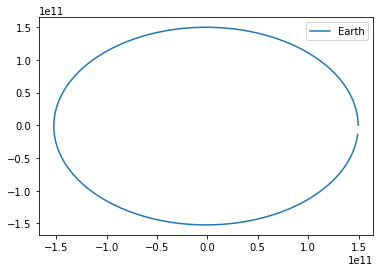
\includegraphics[width=75mm]{figure1.png}
}
\subfloat[OOP Solution]{
  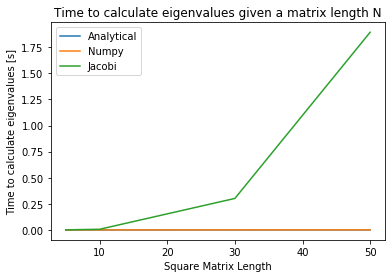
\includegraphics[width=75mm]{figure2.png}
}
\caption{Using both the Euler and Verlet method with and without objects to plot the orbit of Earth for one year using the initial conditions $x_0$ = (1AU , 0), $v_0$ = (0 , $30\times 10^3 m/s$)}
\end{figure} \newline
We additionally compare the run-times and find that (on average over 5 runs):
\begin{table}[ht!]
\centering
 \begin{tabular}{||c c c ||}
 \hline
 
  &  Euler [s] & Verlet [s] \\ [0.5ex] 
 \hline
 \hline
 Mean &  $8.2575\times 10^{-3}$ & $9.1917\times 10^{-3}$ \\ 
 \hline
 STD &  $3.6258\times 10^{-5}$ & $1.4581\times 10^{-4}$ \\
 \hline
 \hline
 
\end{tabular}
\caption{Mean runtimes of the Euler and Verlet solution respectively over 5 runs with standard deviations}
\label{tab1}
\end{table}\newpage
We can now calculate the energy and angular momentum for a circular/elliptical orbit and validate that these values (according to theory) are retained:
\begin{figure}[ht!] \label{fig2}
\centering
\subfloat[All Energies over a year]{
  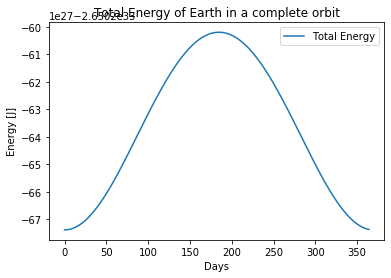
\includegraphics[width=75mm]{figure4.png}
}
\subfloat[Angular momentum over a year]{
  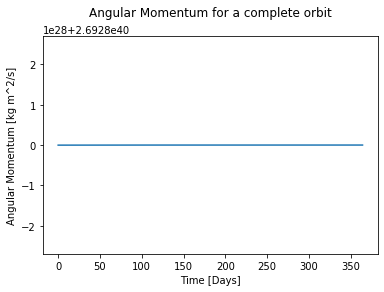
\includegraphics[width=75mm]{figure6.png}
}
\caption{Using the Verlet method to verify that energy and angular momentum is retained during Earths orbit for initial conditions $x_0$ = (1AU , 0), $v_0$ = (0 , $30\times 10^3 m/s$) over a year}
\end{figure}
\begin{figure}[ht!] \label{fig2}
\centering
\subfloat[Energy of elliptical orbit]{
  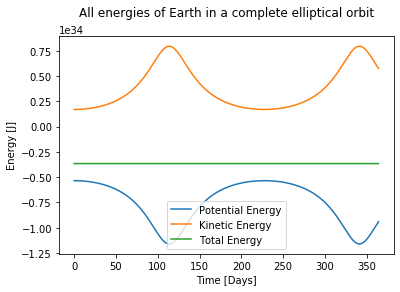
\includegraphics[width=75mm]{figure8.png}
}
\subfloat[Angular momentum of elliptical orbit]{
  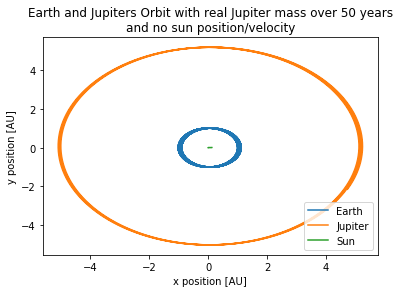
\includegraphics[width=75mm]{figure10.png}
}
\caption{Using the Verlet method to verify that energy is retained during Earths elliptical orbit for initial conditions $x_0$ = (1AU , 0), $v_0$ = (0 , $23.72\times 10^3 m/s$)}
\end{figure} \newpage
We let $\beta$ in $F = \frac{1}{r^\beta}$ approach a breakpoint where we no longer orbit and the body escapes the gravitational pull:
\begin{figure}[ht!]
    \centering
    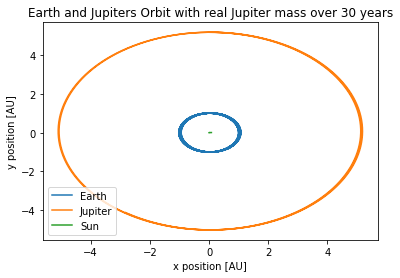
\includegraphics[scale=0.5]{figure7}
    \caption{Orbits for an increasing $\beta$ in $r^\beta$ over a century.}
    \label{fig3}
\end{figure} \newline
Let's now examine the energy and angular momentum of such a system for different values of $\beta$:
\begin{figure}[ht!] \label{fig4}
\centering
\subfloat[Energy of elliptical orbit]{
  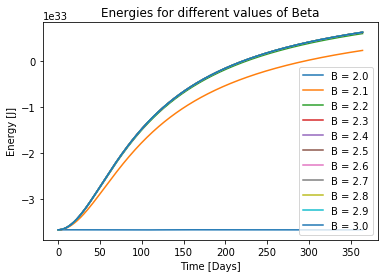
\includegraphics[width=65mm]{figure11.png}
}
\subfloat[Angular momentum of elliptical orbit]{
  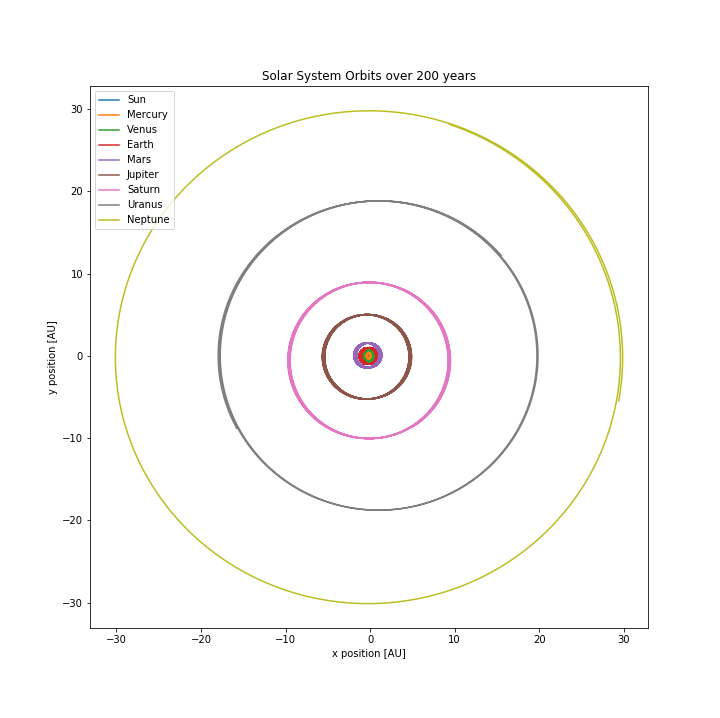
\includegraphics[width=65mm]{figure12.png}
}
\caption{Using the Verlet method with differing $\beta$s to examine that energy is retained during Earths elliptical orbit for initial conditions $x_0$ = (1AU , 0), $v_0$ = (0 , $30\times 10^3 m/s$) over 3 years}
\end{figure} \newpage
Using Equation [\ref{1}] we can calculate the escape velocity in Earths orbit to be:
\begin{equation*}
    v_{velocity} = \sqrt{\frac{2\gamma 2\times10^30}{1AU}} = 42230 \frac{m}{s}
\end{equation*}
Knowing this, we can examine this numerically by letting our initial velocity go from $35\times 10^3 \frac{m}{s}$ to $45\times 10^3 \frac{m}{s}$:
\begin{figure}[ht!]
    \centering
    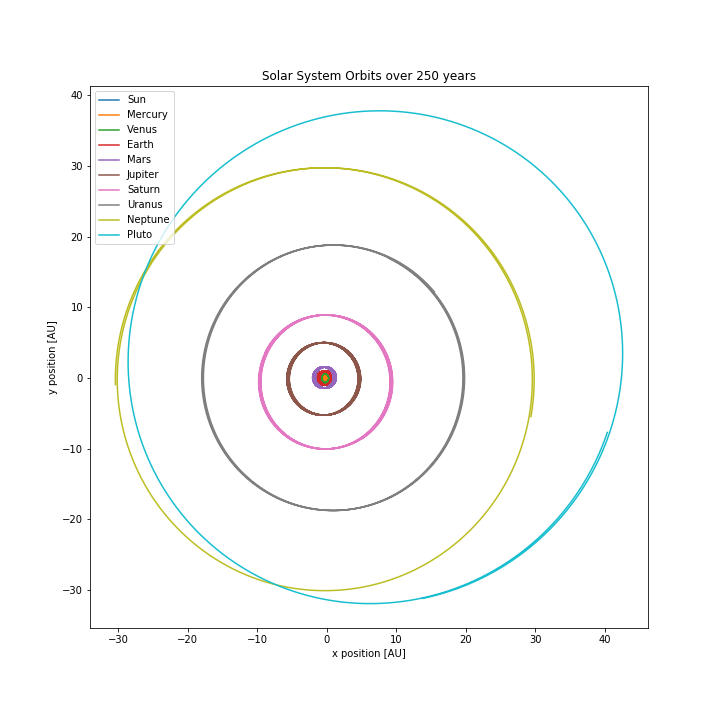
\includegraphics[scale=0.5]{figure13.png}
    \caption{Orbits given different initial velocities.}
    \label{fig5}
\end{figure} \newpage
Let's now examine our system as a whole, we add all 8 planets (and the sun) and plot:
\begin{figure}[ht!] 
\centering
\subfloat[Orbits of all planets in our entire solar system over 200 years]{
  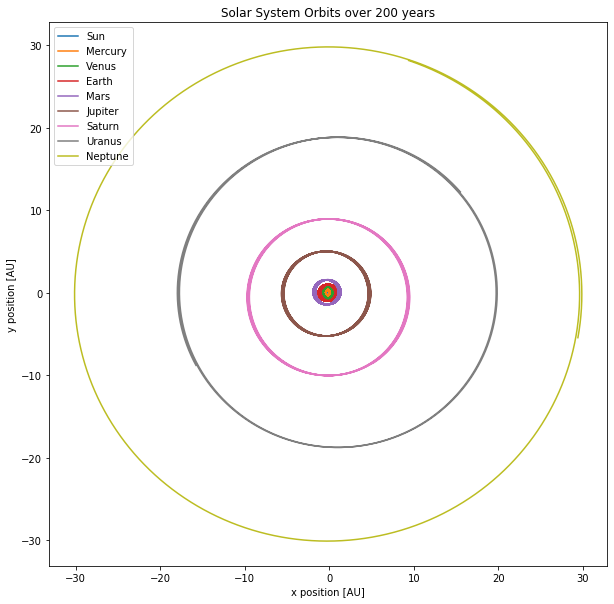
\includegraphics[width=75mm]{figure18.png}\label{fig6}
}
\subfloat[Orbits of the five innermost planets (and the sun)]{
  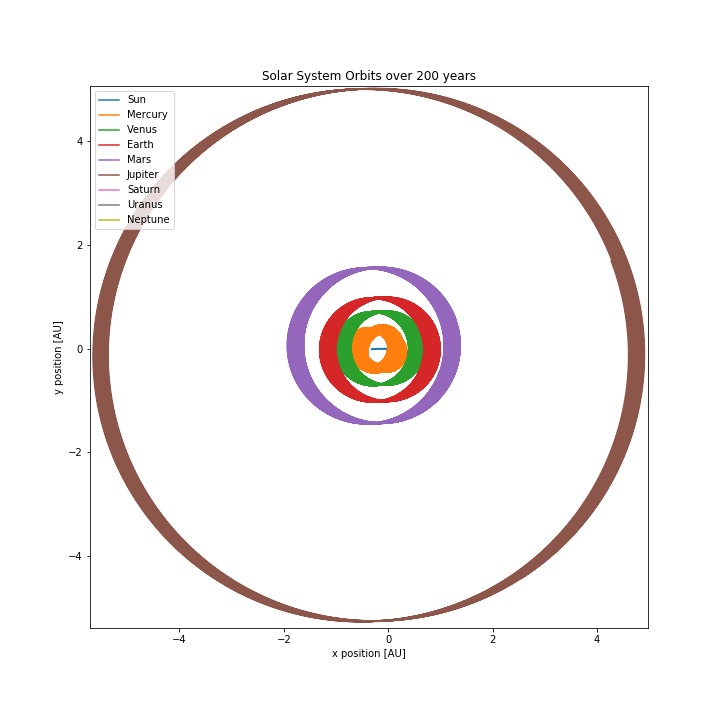
\includegraphics[width=75mm]{figure19.png}
}
\caption{Orbits in our solar system using initial conditions from \cite{NASA}}
\end{figure} \newline
Using \ref{2}, we let Mercury orbit the sun for 100 years, before stopping it at it's Perihelion:
\begin{figure}[ht!]
    \centering
    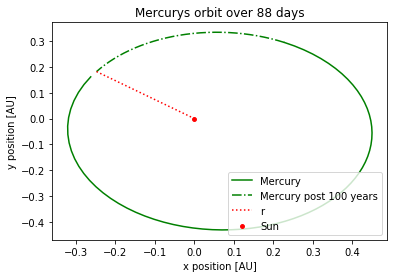
\includegraphics[scale=0.6]{figure20.png}
    \caption{The final 87 days of orbit before we stop to examine it's angle and coordinates.}
    \label{fig7}
\end{figure} \newpage
We find that this angle is $\theta = 2.393194381674042$ rad, and that the annual change in angle is $\Delta \theta_{annual} = -0.024518933385077806$ rad. This means that for one century + the additional days to hit Perihelion, our total theoretical $\theta_{total}$ change is:
\begin{equation*}
    \theta_{total} = \Delta \theta_{annual}*\frac{36500 days + \frac{275 hours}{24 hours}}{88 days} = -3.889792132218641 rad = 2.393393174960945 rad
\end{equation*}
The deviation from the theoretical is then given as:
\begin{equation*}
    \theta_{relativity} = \left |\theta - \theta_{total}\right| = 0.00019879328690297626 rad = 41"
\end{equation*}
which is fairly close to the real answer of $42.98"$
\section{Discussion}
\subsection*{Discussing results}
\subsubsection*{$\beta$-values}
You might've noticed that I instead of letting $\beta$ go from 2 to 3. This is simply because even for a value as low as $\beta = 2.1$, the planet completely broke off from the orbit. As you can see in Figure [\ref{fig3}], for a $\beta$ as small as 2.0275 it breaks off. I obviously haven't been able to figure out why this happens, but I think it might have to do with me using SI units instead of scaling everything accordingly to Astronomical Units, which results in increasingly large $r$ denominators, causing the force to become close to zero.
\subsubsection*{Mercury's Precession}
In regards to the analytical vs. numerical solutions. We find that $\theta_{relativistic}$ =41", which is off by about 4.5\%. This seems pretty massive, but I'm assuming it's perhaps due to some kind of rounding error in Python, as arc seconds scale linearly with radians, but very steeply. As such, all things considered, I wouldn't consider this a bad result.
\newpage
\subsection*{Other discussions}
\subsubsection*{Runtimes and FLOPs}
As shown in Table [\ref{tab1}], our Euler Method was actually faster than it's Verlet counterpart. This is to be expected however, as if we decompose our algorithms we find that: \newline
Euler:
\begin{itemize}
    \item Finding $a_x$,$a_y$ = 2FLOPs
    \item Finding new $v$ = 3FLOPs
    \item Finding new $p$ = 3FLOPs
\end{itemize}
Verlet:
\begin{itemize}
    \item Finding new $p$ = 4 FLOPs
    \item Finding $a_x$, $a_y$ = 2FLOPs
    \item Finding new $v$ = 3FLOPs
\end{itemize}
Note that we've excluded the force function from this calculation, as it is the same across both.
\newline Therefore we find that
\begin{table}[ht!]
\centering
 \begin{tabular}{||c c c ||}
 \hline
 
  &  Euler [s] & Verlet [s] \\ [0.5ex] 
 \hline
 \hline
 Mean &  $8.2575\times 10^{-3}$ & $9.1917\times 10^{-3}$ \\ 
 \hline
 STD &  $3.6258\times 10^{-5}$ & $1.4581\times 10^{-4}$ \\
 \hline
 FLOPs & 8N & 9N \\
 \hline
 \hline
 
\end{tabular}
\caption{Mean runtimes of the Euler and Verlet solution respectively over 5 runs with standard deviations, in addition to the number of FLOPs for each algorithm}
\label{tab2}
\end{table}
\newline \textbf{So why use Verlet when Euler is faster?} \newline
This mostly comes down two main points. Firstly, all the calculations we're doing in this project aren't very costly, meaning runtime doesn't even become an issue, even for something seemingly colossal, like calculating the orbits of the entire solar system over 200+ years. \newline
Secondly, and most importantly, the Verlet method is more accurate than Euler and is symplectic, which means it works very well for systems where energy is conserved. \newpage
\subsubsection*{Stability and corrections}
We were asked to talk about the stability of our solution, which I figured I'd do here.
\newline Let's look at how the Verlet solution behaves for different timesteps $\Delta t$:
\begin{figure}[ht!]
    \centering
    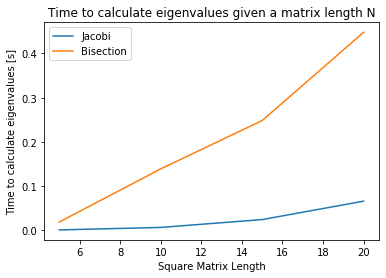
\includegraphics[scale=0.6]{figure3.png}
    \caption{Stability of our solution for four different timesteps. N is scaled accordingly so as to keep the "total time" close to one year}
    \label{fig8}
\end{figure} \newpage
Let's now also look at a three-body system and it's stability:
\begin{figure}[ht!]
    \centering
    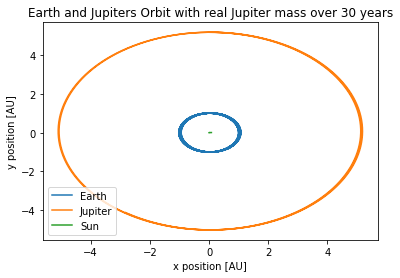
\includegraphics[scale=0.6]{figure14.png}
    \caption{A three-body system using an initialized Earth and Jupiter with the initial conditions: \newline
    Earth: $x_0$ = (1AU , 0), $v_0$ = (0 , $30\times 10^3 m/s$) \newline
    Jupiter: $x_0$ = (0 , 5.2AU), $v_0$ = ($13\times10^3 m/s$, 0)}
    \label{fig8}
\end{figure} \newline
Let's now examine the same system, but with and without the sun initialized so as to make the total momentum 0, and letting the center of mass be (0,0) over 50 years:
\begin{figure}[ht!] \label{fig10}
\centering
\subfloat[Orbit over 50 years with an initialized sun so as to increase the stability of our system]{
  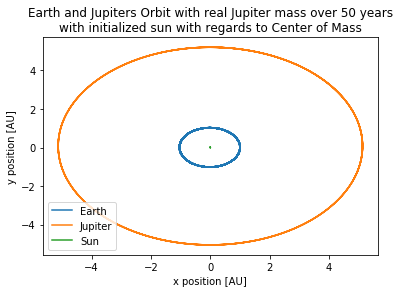
\includegraphics[width=75mm]{figure17.png}
}
\subfloat[Orbit over 50 years without an initialized sun]{
  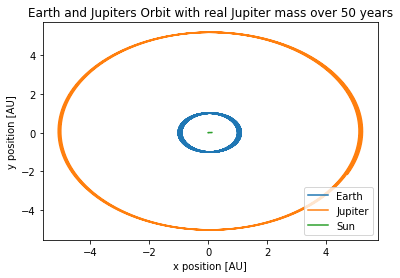
\includegraphics[width=75mm]{figure17b.png}
}
\caption{Two different plots showing the effect of initializing the sun so as to further stabilize our system}
\end{figure} \newline
Notice how the lines on the leftmost plot are significantly thinner than the one on the right. This is because the system we have created for the leftmost plot has close to no drift, meaning it is pretty much a perfect circular orbit, as opposed to the right-side plot which seems to have some drift, and is likely somewhat elliptical in it's orbit.
\newpage
\subsubsection*{Jupiter's mass}
What happens to the stability of our system if we were to amplify the mass of Jupiter? For reference, a normal three-body system consisting of Earth, Jupiter and the sun looks like Figure [\ref{fig8}].
\begin{figure}[ht!] \label{fig12}
\centering
\subfloat[A 30 year orbit with Jupiter having 10$\times$ its normal mass]{
  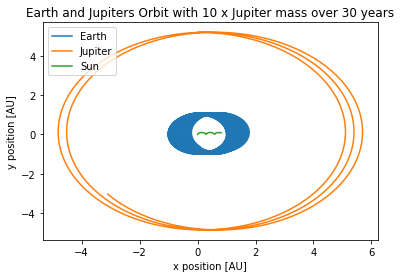
\includegraphics[width=75mm]{figure15.png}
}
\subfloat[A 30 year orbit with Jupiter having 1000$\times$ its normal mass]{
  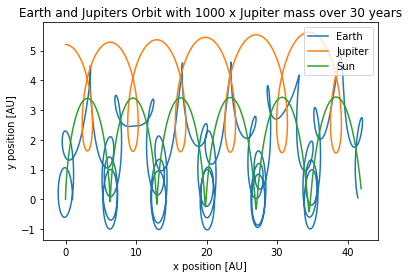
\includegraphics[width=75mm]{figure16.png}
}
\caption{Two different plots showing the effect of Jupiter's mass on Earth and our three-body system.}
\end{figure} \newline
This results is of course to be expected. Jupiter actually almost overtakes the sun in mass when multiplying by 1000, resulting in a very unstable system. Notice how Earth starts orbiting the Sun more like a moon than a planet (except it's sort of the same thing). \newpage
\subsubsection*{Pluto - a potential problem with the model}
I originally wanted to include Pluto in Figure \ref{fig6}, however it deviated severely from it's analytical values, so much so that it finished it's orbit about 50 years prior to when it analytically should. \newline
For reference:
\begin{figure}[ht!]
    \centering
    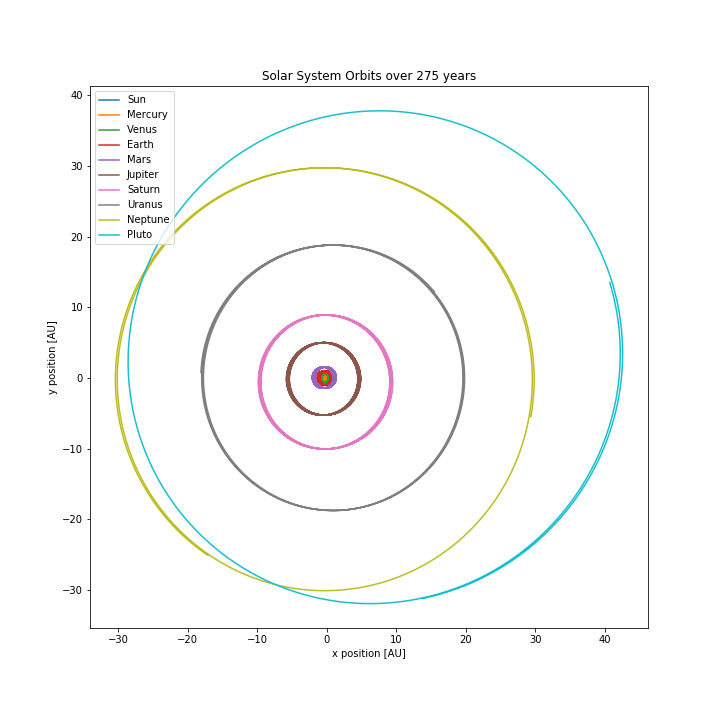
\includegraphics[scale=0.5]{figure18b.png}
    \caption{The same system as \ref{fig6}, this time with Pluto included}
    \label{fig13}
\end{figure} \newline
which was cause for some concern. I wasn't able to deduce what the cause for this would be, but I'm guessing it could be the relative error growing as we increase the amount of time-steps we do, or alternatively that the orbital inclination of Pluto (17.14\degree) is big enough that it causes problems with a two dimensional model.
\section{Conclusion}
In conclusion, we've shown how a multi-body system in space interacts with each other. We've additionally shown that both energy and angular momentum are conserved in both circular and elliptical orbits. \newline
Lastly we've showed that Mercury's relativistic precession can be shown to be 41" at the Perihelion over a period of 100 years.
\bibliographystyle{plainurl}
\bibliography{citations.bib}
\end{document}
